\documentclass[12pt]{article}
\usepackage{graphicx}
\usepackage[usenames,dvipsnames]{xcolor}
\usepackage{color}
\usepackage[spanish, activeacute]{babel}
\usepackage[utf8]{inputenc}  
\usepackage{enumerate}


%codigos: \begin{abstract} \end{abstract} es resumen
%nueva pagina \newpage
%colores predefinidos : white, black, red, green, blue, cyan, magenta, yellow
%\textcolor{blue}{text}
%\color{blue!20!black!30!green}{Prueba} mezcla de colores, conviene manejar solo 2 colores, es mas manejable



\begin{document}
{\centering

\includegraphics[scale=0.5]{imagenes_android/espol.png}
\hspace{0.9in}
\includegraphics[scale=1.6]{imagenes_android/fiec.png}\\
\vspace{0.2in}
{\huge{\textbf{Escuela Superior Polit\'ecnica del Litoral\\\vspace{0.7in}Facultad de Ingenier\'ia en Electricidad y Computaci\'on}}}\\
\vspace{0.7in}
{\LARGE{\textbf{César E. San Lucas Alvarado}}}\\
\vspace{0.1in}
{\Large{csan@espol.edu.ec}}\\
\vspace{0.8in}
{\LARGE \textbf{{Lenguajes de Programaci\'on}}\\
\vspace{0.2in}
{\LARGE \textbf{{2012 - 2013 | II Término}}\\
\vspace{0.5in}

%------------------------------------------------------------------------------------------%
\newpage
\large
\tableofcontents

%------------------------------------------------------------------------------------------%
\newpage
\begin{flushleft}
\section{Android}
\vspace{0.5in}
\normalsize
Este es el primer trabajo de lenguajes de programaci\'on,para el cual las indicaciones fueron las de realizar un proyecto de aplicaci\'on m\'ovil, más espec\'ifico en Android.\\
Hubieron algunas dificultades al principio, era algo nuevo para todos, a\'un no ten\'iamos clara la idea de lo que se har\'ia.\\
Entre algunas ideas, finalmente surgi\'o MY TWIN, algo que realmente nos pareci\'o novedoso y con alguna utilidad que se puede agregar a un dispositivo m\'ovil.\\
Se trabajo bastante con los recursos del tel\'efono y se hizo mucho \'enfasis en la proyecci\'on de tener un dispositivo con todo personalizado.
\begin{center}
\vspace{0.5in}

\includegraphics[scale=0.7]{imagenes_android/logo}
\end{center}
\end{flushleft}

%------------------------------------------------------------------------------------------%
\newpage
\begin{flushleft}
\subsection{Introducci\'on}

\normalsize
MY TWIN una aplicaci\'on dirigida a toda clase de usuario mediante la cual podr\'as crear tu propio avatar, el cual se convertir\'a en tu asesor personal de tareas.

Una aplicaci\'on la cual jugar\'a con los estados de \'animo de tu avatar, los cuales estar\'an definidos por las diferentes tareas que cumplir\'a. Esto es que la aplicaci\'on no solo ser\'a para entretenimiento tendr\'a una funcionalidad que buscar\'a ayudar al usuario de una manera diferente, entretenida y personalizada.\\

\subsection{Idea}
\subsubsection{Problem\'atica}
Muchas veces tenemos nuestro celular o cualquier dispositivo m\'ovil en el cuál podemos programar para que nos notifique o nos recuerde algunas tareas, pero eso es todo lo que hace.\\
Buscabamos entonces una funcionalidad extra al tel\'efono y que a la vez sea agradable al ususario.\\
Todo comenz\'o con una lluvia de ideas, donde algunas fueron muy simples y de poca utilidad y otrass en cambio eran muy complicadas y sin prestar el mayor benefecio, as\'i finalmente surgi\'o My Twin, idea que nos agrad\'o por que era posible de llevar a la realidad y adem\'as mejorar\'ia la funcionalidad de nuestro dispositivo m\'ovil.\\
My Twin como un entretenido gemelo virtual.\\
\begin{center}
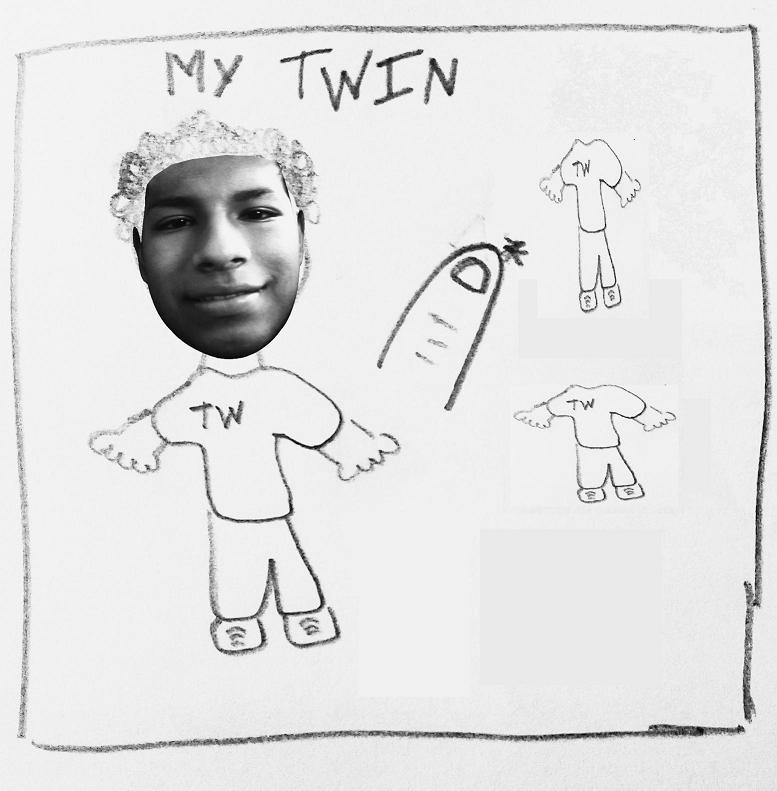
\includegraphics[scale=0.3]{imagenes_android/bosquejoI1}
\end{center}

\end{flushleft}


%------------------------------------------------------------------------------------------%
\newpage
\begin{flushleft}
\subsubsection{Dise\~no}
\normalsize
El primer borrador fue trabajado en hojas con dibujos a mano, debido a que My Twin no era una sola pantalla est\'atica, sino que tiene algunas pantallas en la cual va cada una de las funciones.\\
Se dibujo algunos probables dise\~nos hasta llegar al que se tom\'o como modelo el siguiente.\\
\vspace{0.3in}
\begin{center}
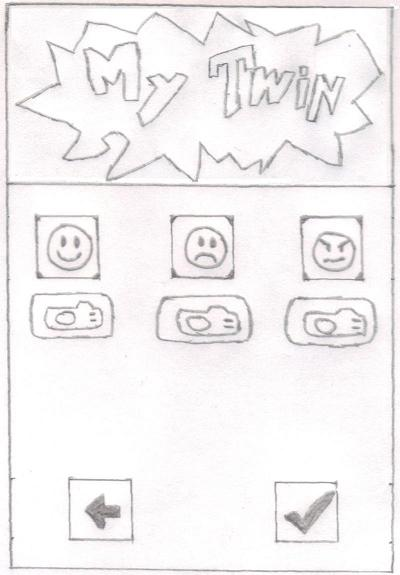
\includegraphics[scale=0.42]{imagenes_android/Twin1}
\hspace{0.3in}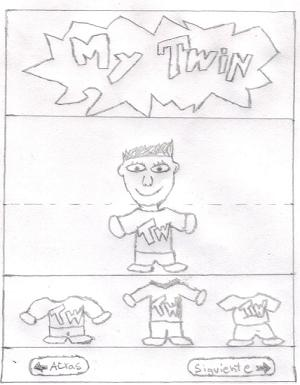
\includegraphics[scale=0.65]{imagenes_android/Twin2}\vspace{0.1in}
\end{center}
\begin{center}
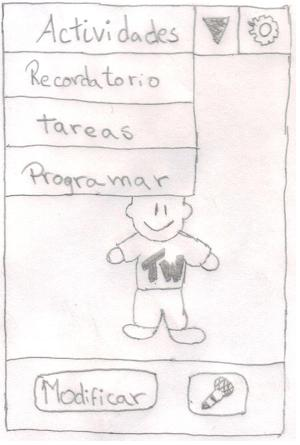
\includegraphics[scale=0.6]{imagenes_android/Twin3}
\end{center}


\end{flushleft}


%------------------------------------------------------------------------------------------%
\newpage
\begin{flushleft}
\subsection{My Twin}
\subsubsection{Descripci\'on General}
\vspace{0.2in}
\normalsize
My Twin es una aplicaci\'on para dispositivos móviles: \\\vspace{0.2in}\textbf{My Twin es divertido y original.\\
\vspace{0.1in}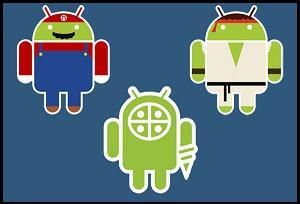
\includegraphics[scale=0.6]{imagenes_android/3.jpg}\\
\begin{center}
\vspace{0.1in}My Twin es realista.\\
\vspace{0.1in}
\includegraphics[scale=0.6]{imagenes_android/droid.jpg}\\
\end{center}
\begin{flushright}
\vspace{0.1in}My Twin es amigable con el usuario.\\
\vspace{0.1in}
\includegraphics[scale=0.6]{imagenes_android/amigableU.jpg}\\
\end{flushright}
}


\end{flushleft}

%------------------------------------------------------------------------------------------%
\newpage
\begin{flushleft}
\subsection{Funcionamiento (Manual de Usuario)}
\subsubsection{Pantalla Principal}
\vspace{0.1in}
\normalsize
Pantalla Principal de My Twin, presionando en entrar, nos llevar\'a a la siguiente pantalla, si no tenemos aun creado el Twin, iremos a la pantalla de crear Twin, si ya lo tenemos, iremos directamente a la pantalla donde esta el menu y nuestro Twin.

\begin{center}
\vspace{0.3in}Pantalla Principal de inicio.\\
\vspace{0.3in}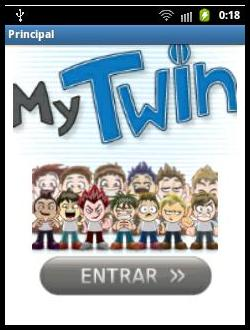
\includegraphics[scale=1.2]{imagenes_android/PPrincipal}\\
\end{center}

\newpage
\subsubsection{Creaci\'on de Twin}
\vspace{0.1in}
Estas son las dos pantallas de creaci\'on del gemelo virtual, la primera es donde realizamos las fotos para la cara, d\'andole as\'i realismo; la segunda es para escoger un cuerpo, el cual le pone el lado original y divertido,donde todo es personalizable. \\
\begin{center}
\vspace{0.5in}
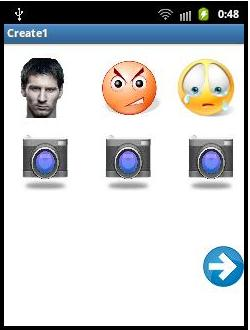
\includegraphics[scale=1.0]{imagenes_android/create1.jpg}
\hspace{0.1in}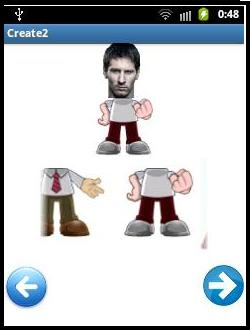
\includegraphics[scale=1.0]{imagenes_android/create2.jpg}
\end{center}


%------------------------------------------------------------------------------------------%
\newpage
\subsubsection{Menu Tareas}
\vspace{0.1in}
Luego de tener creado nuestro gemelo virtual, podemos ver el menu de tareas, el cual ser\'a la pantalla que veremos cada vez que entremos a la aplicaci\'on, el funcionamiento es sencillo, cuando vemos el menu se muestra en claras palabras lo que encontraremos al ingresar ah\'i.\\\vspace{0.2in}
\textbf{Tareas:} Nos llevar\'a a la pantalla de tareas, en la cual podremos programar los recordatorios de manera personalizada.\\\vspace{0.1in}
\textbf{Modificar:} Nos llevar\'a de regreso a la pantalla de creaci\'on de Twin, para que podamos realizar las modificaciones que queremos.\\\vspace{0.1in}
\textbf{Programar:} Nos permitir\'a programar el tel\'efono para casos especiales, como por ejemplo el ahorro de energ\'ia.\\

\begin{center}
\vspace{0.5in}
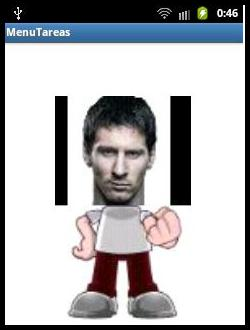
\includegraphics[scale=1.0]{imagenes_android/MenuTareas1.jpg}
\hspace{0.1in}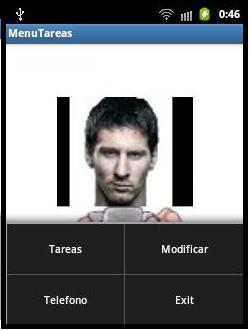
\includegraphics[scale=1.0]{imagenes_android/MenuTareas2.jpg}
\end{center}

%------------------------------------------------------------------------------------------%
\newpage
\subsubsection{Nueva Tarea}
\vspace{0.1in}
Aqu\'i podemos ver tres botones que hacen referencia al sonido, adem\'as de un reloj.\\
El funcionamiento es muy sencillo. En el reloj ponemos la hora que queremos establecer para recordar y los botones de grabacion funcionan así: uno para grabar, otro para detener y otro para reproducir la grabaci\'on.\\
Es importante recalcar que sin grabaci\'on no se puede avanzar, porque esto es parte del objetivo de buscar la originalidad, por esto es necesario que la tarea la recuerde con nuestra voz.\\
La otra parte importante es que podemos realizar tantas grabaciones como queramos, pues solo se escoger\'a la \'ultima, como parte de darle facilidad al ususario para que no tenga que iniciar el proceso nuevamente, esto se realiza de una manera sencilla en el mismo momento.\\

\begin{center}
\vspace{0.5in}
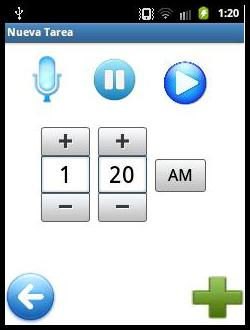
\includegraphics[scale=1.0]{imagenes_android/NuevaTarea1.jpg}
\hspace{0.1in}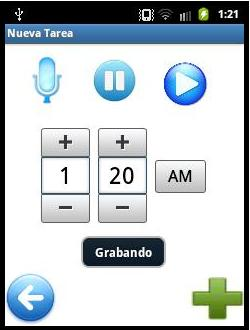
\includegraphics[scale=1.0]{imagenes_android/NuevaTarea2.jpg}
\end{center}

%------------------------------------------------------------------------------------------%
\newpage
\subsubsection{Programar}
\vspace{0.1in}
Esta funci\'on de la aplicaci\'on nos permite manejar recursos mas internos del dispositivo m\'ovil, de modo que se pueda programar su funcionamiento y manejarlo con un tiempo definido.\\

\begin{center}
\vspace{0.6in}
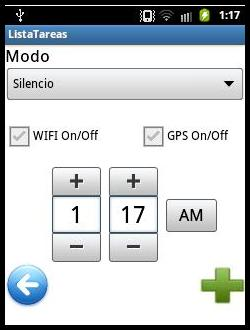
\includegraphics[scale=1.2]{imagenes_android/Programar1.jpg}
\end{center}

%------------------------------------------------------------------------------------------%
\newpage
\subsection{Conclusión}
Consideramos que logramos una aplicaci\'on completa que rompe la monoton\'ia de alarmas con tonos ruidosos
por una grabaci\'on de voz realizada por el usuario; aparte de eso la aplicaci\'on nos permite controlar los recursos 
b\'asicos del telefono.
\subsection{Experiencias}
Realizar este trabajo no ha sido algo f\'acil, tuvimos varios inconvenientes. Al principio no encontrabamos la idea que nos ayudar\'ia a realizar este proyecto, luego vimos que este entorno de trabajo era diferente a lo que anteriormente hemos realizado, lo bueno es que contabamos con buenas bases de programaci\'on lo cual facilitaba un poco el entendimiento de lo nuevo que estabamos por ver.\\
En general el grupo siempre estuvo en contacto, de ese modo siempre se avanzaba en el trabajo, algunas veces tuvimos que trabajar hasta muy tarde por la noche, pero, a\'un as\'i vali\'o la pena, porque el trabajo se present\'o completo cumpliendo las expectativas que ten\'iamos acerca de la aplicaci\'on, adem\'as que ayud\'o a unir al grupo en amistad, pues cada problema que se presentaba se resolv\'ia realizando una reuni\'on ya sea f\'isicamente o por medio del internet.\\
Muchas de las cosas hubo que investigarlas puesto que esta era una experiencia nueva para todos y ninguno ten\'ia el conocimiento de lo que realizar\'iamos. Para resolver de manera mas eficiente, cada uno investigaba una parte y luego en reuni\'on expresabamos lo que hab\'iamos encontrado; en conjunto aprendimos cada uno de la experiencia del otro y de la informaci\'on que le toco buscar.\\
El entorno de trabajo para Android fue un poco complicado, pero sirvi\'o para darnos un empuje a lo que ser\'ian los otros proyectos de la materia, pudimos ver desde otra perspectiva la programaci\'on utilizando otras herramientas para trabajar; el hecho de tener exposiciones peri\'odicas del avance del proyecto nos presionaba precisamente a eso, que el proyecto estuviese en marcha, de este modo no nos atrasamos ni en terminar el trabajo ni en presentarlo.\\
\vspace{0.1in}Finalmente toda experiencia es y ha sido enriquecedora desde el punto de vista de conocimiento.

\end{flushleft}

%------------------------------------------------------------------------------------------%
\newpage
\begin{flushleft}
\section{Phyton}
\vspace{0.3in}
\subsection{Introducci\'on}
\normalsize
``Entrega tu Tarea! Es un divertido juego, con orientación educativa, puesto que de una forma entretenida, los niños podrán ejercitar su mente, sus habilidades matemáticas a través de un sano juego.
\newline
\newline
``Entrega tu Tarea tendrá como usuarios niños de jardin (4-5 años)  y de escuela (7-12 años). El objetivo es que el usuario vaya estructurando una tarea que consta de 3 partes: habilidad con la memoria, habilidades matemáticas, y habilidades visuales; otro objetivo es que el usuario pueda seguir correctamente las instrucciones que se le dan por medio de un audio.
\newline
\newline
Con una serie de audios e imágenes el usuario manejará facilmente este juego, y empezará a relacionar tareas diarias escolares con algo entretenido y práctico
\newline
\newline
Este juego está desarrollado en Python utilizando la librería Pygame, como herramientas adicionales se utilizó Adobe Photoshop para la creación de imágenes y Audacity para la creación de audios.
\vspace{0.1in}

%------------------------------------------------------------------------------------------%
\subsection{Funcionalidades (Manual de Usuario)}

\normalsize
Entrega tu Tarea cuenta con muchas funcionalidades. Es un juego en el que con el paso de los niveles el usuario obtendrá cada vez mas habilidades.
\newline
\newline
La primera funcionalidad es la parte llamada "Memoriza", en esta parte el usuario tendrá que escuchar un audio con una secuencia de letras y números y despues ingresar correctamente dicha secuencia por teclado.
\newline
\newline
La segunda funcionalidad es la "Tarea matemática"  que consta de un ejercicio matemático conforme al nivel estudiantil y años que tiene el usuario, datos que se piden en el transcurso del juego.	
\newline
\newline	
Finalmente si el usuario ha respondido correctamente las tareas anteriores, tendrá que pasar por un divertido juego en el que tendrá que superar una serie de obtaculos para poder entregar su tarea exitosamente.
\newline
\newline
En el transcurso del juego, el usuario tendrá que seguir las instrucciones proporcionadas en audio.
\newline
\newline
El juego está hecho de forma que el usuario ingrese su nivel educativo(Jardín o escuela) y su edad; con estos datos, el programa escogerá que tipo de ejercicios matemáticos son los adecuados para la tarea.

%------------------------------------------------------------------------------------------%
\subsubsection{Inicio del Juego}
\vspace{0.1in}
Inicio del juego. Escoja la opción que desee. Si desea jugar directamente, escoja por medio de las direccionales qué nivel educativo tiene y presione enter. Si desea conocer acerca de los creadores del programa, diríjase a la opción Creadores y presione enter
\vspace{0.3in}

	\begin{center}
		\begingroup
			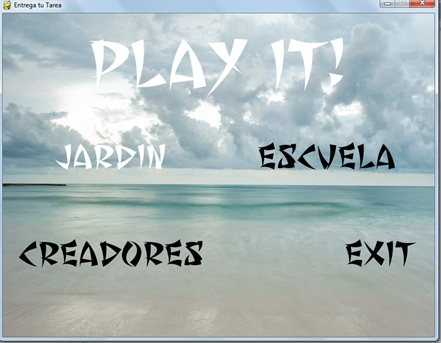
\includegraphics[width=0.8\textwidth]{imagenes_usuario/inicio.jpg}
		\endgroup
	\end{center}

%------------------------------------------------------------------------------------------%
\subsubsection{Escoger el nivel}
\vspace{0.1in}
Al escoger el nivel jardin o el nivel escuela, escuchará un audio con instrucciones. Esta es la tarea de "Memoria", memorice la secuencia e ingresela por teclado, al terminar de ingresar dicha secuencia presione la tecla F5.

	\begin{center}
		\begingroup
			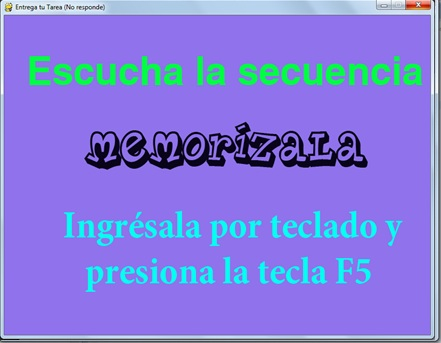
\includegraphics[width=0.6\textwidth]{imagenes_usuario/memoriza}
		\endgroup
	\end{center}
\vspace{0.2in}
Inmediatamente saldrá un audio junto con una imagen que pedirán su edad, ingrésela por medio del teclado y cuando haya terminado presione la tecla F3

	\begin{center}
		\begingroup
			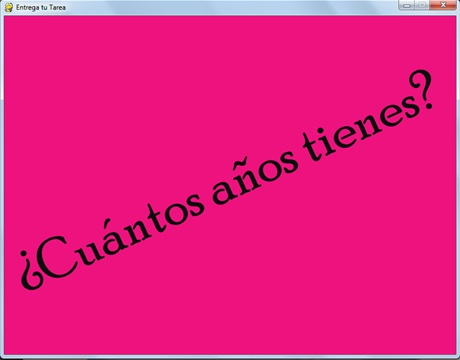
\includegraphics[width=0.6\textwidth]{imagenes_usuario/anios.jpg}
		\endgroup
	\end{center}
%------------------------------------------------------------------------------------------%
\subsubsection{Resolver la tarea}
\vspace{0.1in}
Después de haber ingresado su edad, pasará a la "Tarea Matemática", escuchará una serie de instrucciones y aparecerá una imagen con un ejercicio de matemáticas conforme al nivel educativo que ingresó al comienzo (Jardín o escuela) y de acuerdo a la edad que proporcionó anteriormente.
Resuelve el ejercicio, no hay límite de tiempo. Si se está seguro de la respuesta ingrésela por medio del teclado y presione la tecla F4.
Si la respuesta es incorrecta, escuchará un audio que le dirá que tiene una segunda oportunidad. El límite de equivocaciones es 3, si se equivoca mas de 3 veces, perderá.
\vspace{0.4in}
	\begin{center}
		\begingroup
			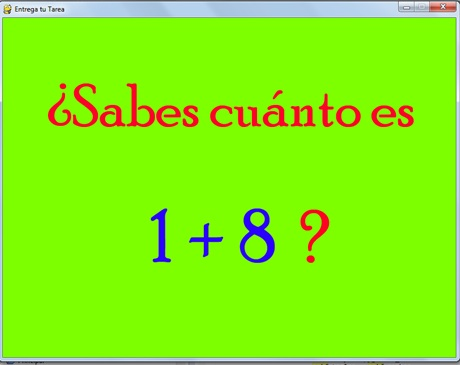
\includegraphics[width=0.8\textwidth]{imagenes_usuario/ejercicio.jpg}
		\endgroup
	\end{center}
\vspace{0.5in}
%------------------------------------------------------------------------------------------%
\subsubsection{Jugando}
\vspace{0.1in}
Si se contestó correctamente, se pasará al juego, en el que se tendrá que pasar una serie de obstáculos para poder entregar su tarea exitosamente.
Escuchará las instrucciones respectivas del juego.
Muévase con las teclas direccionales (derecha: mover derecha, izquierda: mover izquierda, arriba: saltar) y dispare a las caritas felices con la tecla 1.
\vspace{0.4in}
	\begin{center}
		\begingroup
			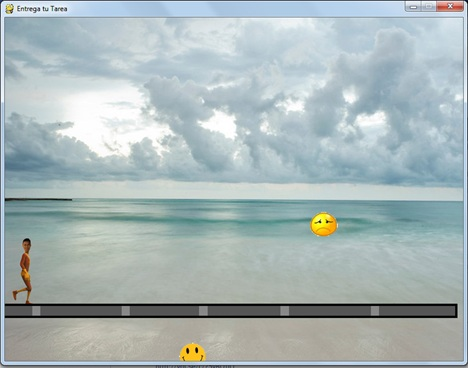
\includegraphics[width=0.6\textwidth]{imagenes_usuario/juego1.jpg}
		\endgroup
	\end{center}
\vspace{0.3in}
Si se realizaron todas las tareas completamente, el usuario habrá ganado y entregado su tarea con exito!
%------------------------------------------------------------------------------------------%
\newpage
\subsection{Nuevo projecto}
\vspace{0.1in}
Debido a que nuestro juego no cumplía extrictamente con las especificaciones de que se debía realizar un juego tipo aventura solo con audio sin contar de ninguna interfaz gráfica, en el cuál únicamente las instrucciones deberían ser dadas por audio y el usuario tomar acciones únicamente con el teclado para continuar en diferentes eventos de la aventura. Por lo cuál decidimos corregir el mismo.

\subsubsection{La Aventura de Sakura}
\vspace{0.1in}
Sakura es una niña muy extrovertida, siempre risueña, y buena estudiante.
Un día Sakura queda sola en su casa, su padre y su hermano se habían ido a trabajar; de pronto escucha un sonido extraño en el sótano de su casa. Sakura se asustó mucho, tenía que tomar una decisión: \\
1.	Llamar a la policía\\
2.	Ir a averiguar que sucedía ella misma\\
Si escoges la opción 1:\\
Sakura llama a la policía. La policía llega en 45 minutos como es costumbre en Ecuador, y al entrar en su casa se dan cuenta que no había nada en el sótano. Sakura se ganó una multa porque se consideró que estaba jugando con el tiempo de la policía.\\
Si escoges la opción 2:\\
Sakura cogió su bastón de porrista y se dirigió en silencio al sótano, abrió lentamente la puerta y estaba muy oscuro
Sakura aún no está segura si bajar al sótano.\\
1.	Sakura se retracta y llama a la policía\\
2.	Sakura se llena se valor y va a averiguar que sucede\\
Si escoges la opción 1:\\
Sakura llama a la policía. La policía llega en 45 minutos como es costumbre en Ecuador, y al entrar en su casa se dan cuenta que no había nada en el sótano. Sakura se ganó una multa porque se consideró que estaba jugando con el tiempo de la policía.\\
Si escoges la opción 2:\\
Sakura baja lentamente las escaleras, recorre el sótano y se da cuenta que no había nadie. Pero de pronto se dio cuenta que misteriosamente uno de los libros que se encontraban en el sótano brillaba intensamente; que hará Sakura?\\
1.	Sakura se retracta y llama a la policía\\
2.	Sakura abre el libro y averigua de que se trata este misterio\\

Si escoges la opción 1:\\
Sakura llama a la policía. La policía llega en 45 minutos como es costumbre en Ecuador, y al entrar en su casa se dan cuenta que no había nada en el sótano. Sakura se ganó una multa porque se consideró que estaba jugando con el tiempo de la policía.\\

Si escoges la opción 2:\\
Sakura abre el libro y una fuerte ráfaga de viento sale fuertemente desde el libro. Una serie de cartas salen volando y atraviesan el techo y se dispersen por todo el cielo, sin embargo sakura pudo tomar 2 en su mano. Las cartas viento y agua. De repente un simpático personaje entra en escena y le dice a Sakura.  Yoo soy el guardián de este libro, mi nombre es Kerberos quien eres tuu?
Sakura le responde con una pregunta y le dice: Tú eras el que hacías ruido con tus ronquidos?
Kerberos le responde avergonzado: yo no ronco aunque he estado dormido hace 400 años. Mi deber es proteger las cartas que ves aquí, señalando el libro, pero no había ya ninguna carta, todas habían volado ya.
Sakura le cuenta a kero que las cartas salieron volando.
Kerberos pega un gritoo al cielo y le dice a Sakura: Ohhh nooo!! Ahora es tu misión recolectar nuevamente las llamadas cartas clow, ya que si estas están sueltas pueden destruir el mundo.\\
Sakura se queda helada, debe tomar una decisión:\\
1.	Rechaza la misión y deja que el mundo se destruya poco a poco.\\
2.	Acepta la misión y recolecta todas las cartas, lo cual es una misión muy peligrosa.\\
Si escoges la opción 1:\\
El mundo entra en caos y nadie puede hacer nada, el fin del mundo ha llegado por la falta de valentía de Sakura. Fin\\
Si escoges la opción 2:\\
La siguiente noche cerca de la casa de sakura hubo un incendio que ni siquiera los bomberos podían apagar. Kerberos que se encontraba junto a sakura, sintió la presencia de una carta Clow, él estaba seguro que ese incendio tuvo que ser ocasionado por algún poder extraño ya que no se trataba de un incendio normal.
Kerberos le dice a Sakura que su misión inicia en ese momento. Sakura contaba con 2 cartas clown: Agua, viento y vuelo.
Tenía que valerse de alguna de estas cartas para poder vencer al terrible Fuego.
Primero tenía que llegar al lugar del incendio. Como llegaría?\\
1.	Sakura llega al lugar con los patines con los que siempre se moviliza al colegio aunque  quizás cuando llegue ya no se pueda hacer nada.\\
2.	Sakura le tiene pánico a las alturas. Pero podía utilizar la carta del vuelo para llegar hasta allá.\\
Si escoges la opción 1:\\
Cuando llega sakura el fuego se extendió demasiado, muchas personas han muerto, y ya no se puede hacer nada, Sakura fracasó en su misión. Y las cartas se apoderaron del mundo entero. Fin\\
Si escoges la opción 2:\\
1.	Sakura utiliza la carta vuelo y llega rápidamente al incendio. Debe de tomar una decisión para poder extinguir el fuego:\\
1.	Sakura utiliza la carta agua.\\
2.	Sakura utiliza la carta viento\\

Si escoges la opción 1:\\
1.	Sakura utiliza la carta Agua y logra vencer el fuego. Sakura cumplió exitosamente su misión y tiene una carta más que podrá utilizar en sus futuras misiones.\\
Si escoges la opción 2:\\
2.	Sakura utiliza el viento, y este hace que el fuego se haga aún más grande; el fuego se extendió demasiado, muchas personas han muerto, y ya no se puede hacer nada, Sakura fracasó en su misión. Y las cartas se apoderaron del mundo entero. Fin\\


%------------------------------------------------------------------------------------------%

\subsection{Conclusiones}
\vspace{0.1in}
Cuando empezamos a estudiar Python, al iniciar este proyecto, nos encantó este lenguaje, nos parecio sencillo y totalmente completo; lo que nos parecip más interesante es la facilidad en la sintaxis del lenguaje, no es muy estricto como los otros lenguajes que dan mil errores por la falta de un punto y coma; sin embargo python se guía de manera excelente solo con identación; aunque nunca le habíamos puesto tanto interés en la identación, ahora lo hacemos  y lo haremos en cualquier lenguajes aunque no se trate de python.

\newpage
\subsection{Experiencias}
\vspace{0.1in}
La librería de Pygame, me parecio increíbles por todas las funcionalidades que éste ofrece.
Al utilizar un ciclo while los juegos realizados en pygame, el manejar la actualizacion de los diferentes estados del juego (interfaz grafica) resultó un poco tedioso realizar el cambio de pantallas de nuestra aplicación.
\newline
\newline
El manejo de Sprites y GroupSprites disponibles en pygame nos resulto "mágico" debido a que esta clases nos proveen muchas funcionalidades muy interesantes como por ejemplo para dibujar un objeto en pantalla que herede de Sprite tan solo es necesario utilizar "el rectángulo e imagen del objeto" y el uso GroupSprites son un conjunto de Sprites y para dibujarlos hace uso de cada uno de los rectángulos e imagenes de los Sprites que se encuentran en el grupo, 
por esto darla apariencia de movimiento e interaccion del objeto tan solo fue necesario actualizar su posicion en pantalla puntos (x,y) y con estos actualizar el rectángulo del objeto.
\newline
\newline
Al comienzo del proyecto parecía un poco exagerado esto de hacer un “Video Juego” pero en el transcurso del proyecto esto se fue convirtiendo en una tarea más fácil y entretenida. Nos gustó mucho programar un Video Juego, espero mejorarlo con el tiempo.
En resumen fue una linda experiencia trabajar en este proyecto.
\newline
\newline
La ejecución del nuevo projecto resultó fácill debido a que el uso de cada funcionalidad que se solicitaba en el mismo la sabíamos implementar porque lo habíamos realizado en el projecto previo el cual era más complejo debido a que era un completo video juego a mediana escala.
\end{flushleft}




\end{document}